\documentclass{standalone}
\usepackage{tikz}
\usetikzlibrary{positioning}

\begin{document}

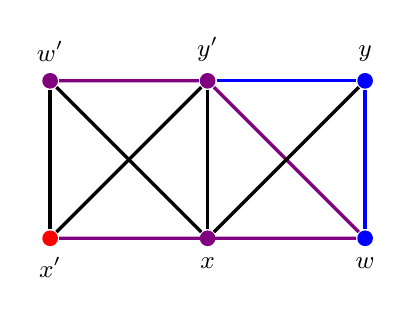
\begin{tikzpicture}[
    node/.style={circle, fill=#1, inner sep=2pt},
    every label/.style={font=\small},
    thick,
    >=stealth
]

% Define node coordinates
\node[node=violet,label=above:$w'$] (w') at (0,2) {};
\node[node=red,label=below:$x'$] (x') at (0,0) {};
\node[node=violet,label=below:$x$] (x) at (2,0) {};
\node[node=violet,label=above:$y'$] (y') at (2,2) {};
\node[node=blue,label=above:$y$] (y) at (4,2) {};
\node[node=blue,label=below:$w$] (w) at (4,0) {};

% Draw edges
\draw[blue, very thick] (w') -- (y') -- (y) -- (w) -- (x);
\draw[red, very thick] (x') -- (x) -- (w);
\draw[black, very thick] (w') -- (x') -- (x) -- (y');
\draw[violet, very thick] (w') -- (y') -- (w) -- (x');

% Add diagonal edges
\draw[black, very thick] (w') -- (x);
\draw[black, very thick] (x') -- (y');
\draw[black, very thick] (x) -- (y);

\end{tikzpicture}

\end{document}